\section{Introduction}
\label{sec:Introduction}

\subsection{The Standard Model}
\label{sec:StandardModel}

The Standard Model (SM) is a theory that describes the elementary particle (fermions and bosons) and their interactions via three fundamental forces. The SM elementary particles are illustrated in Figure~\ref{fig:SMParticles} and described in more detail below.

\begin{figure}[h]
  \centering
  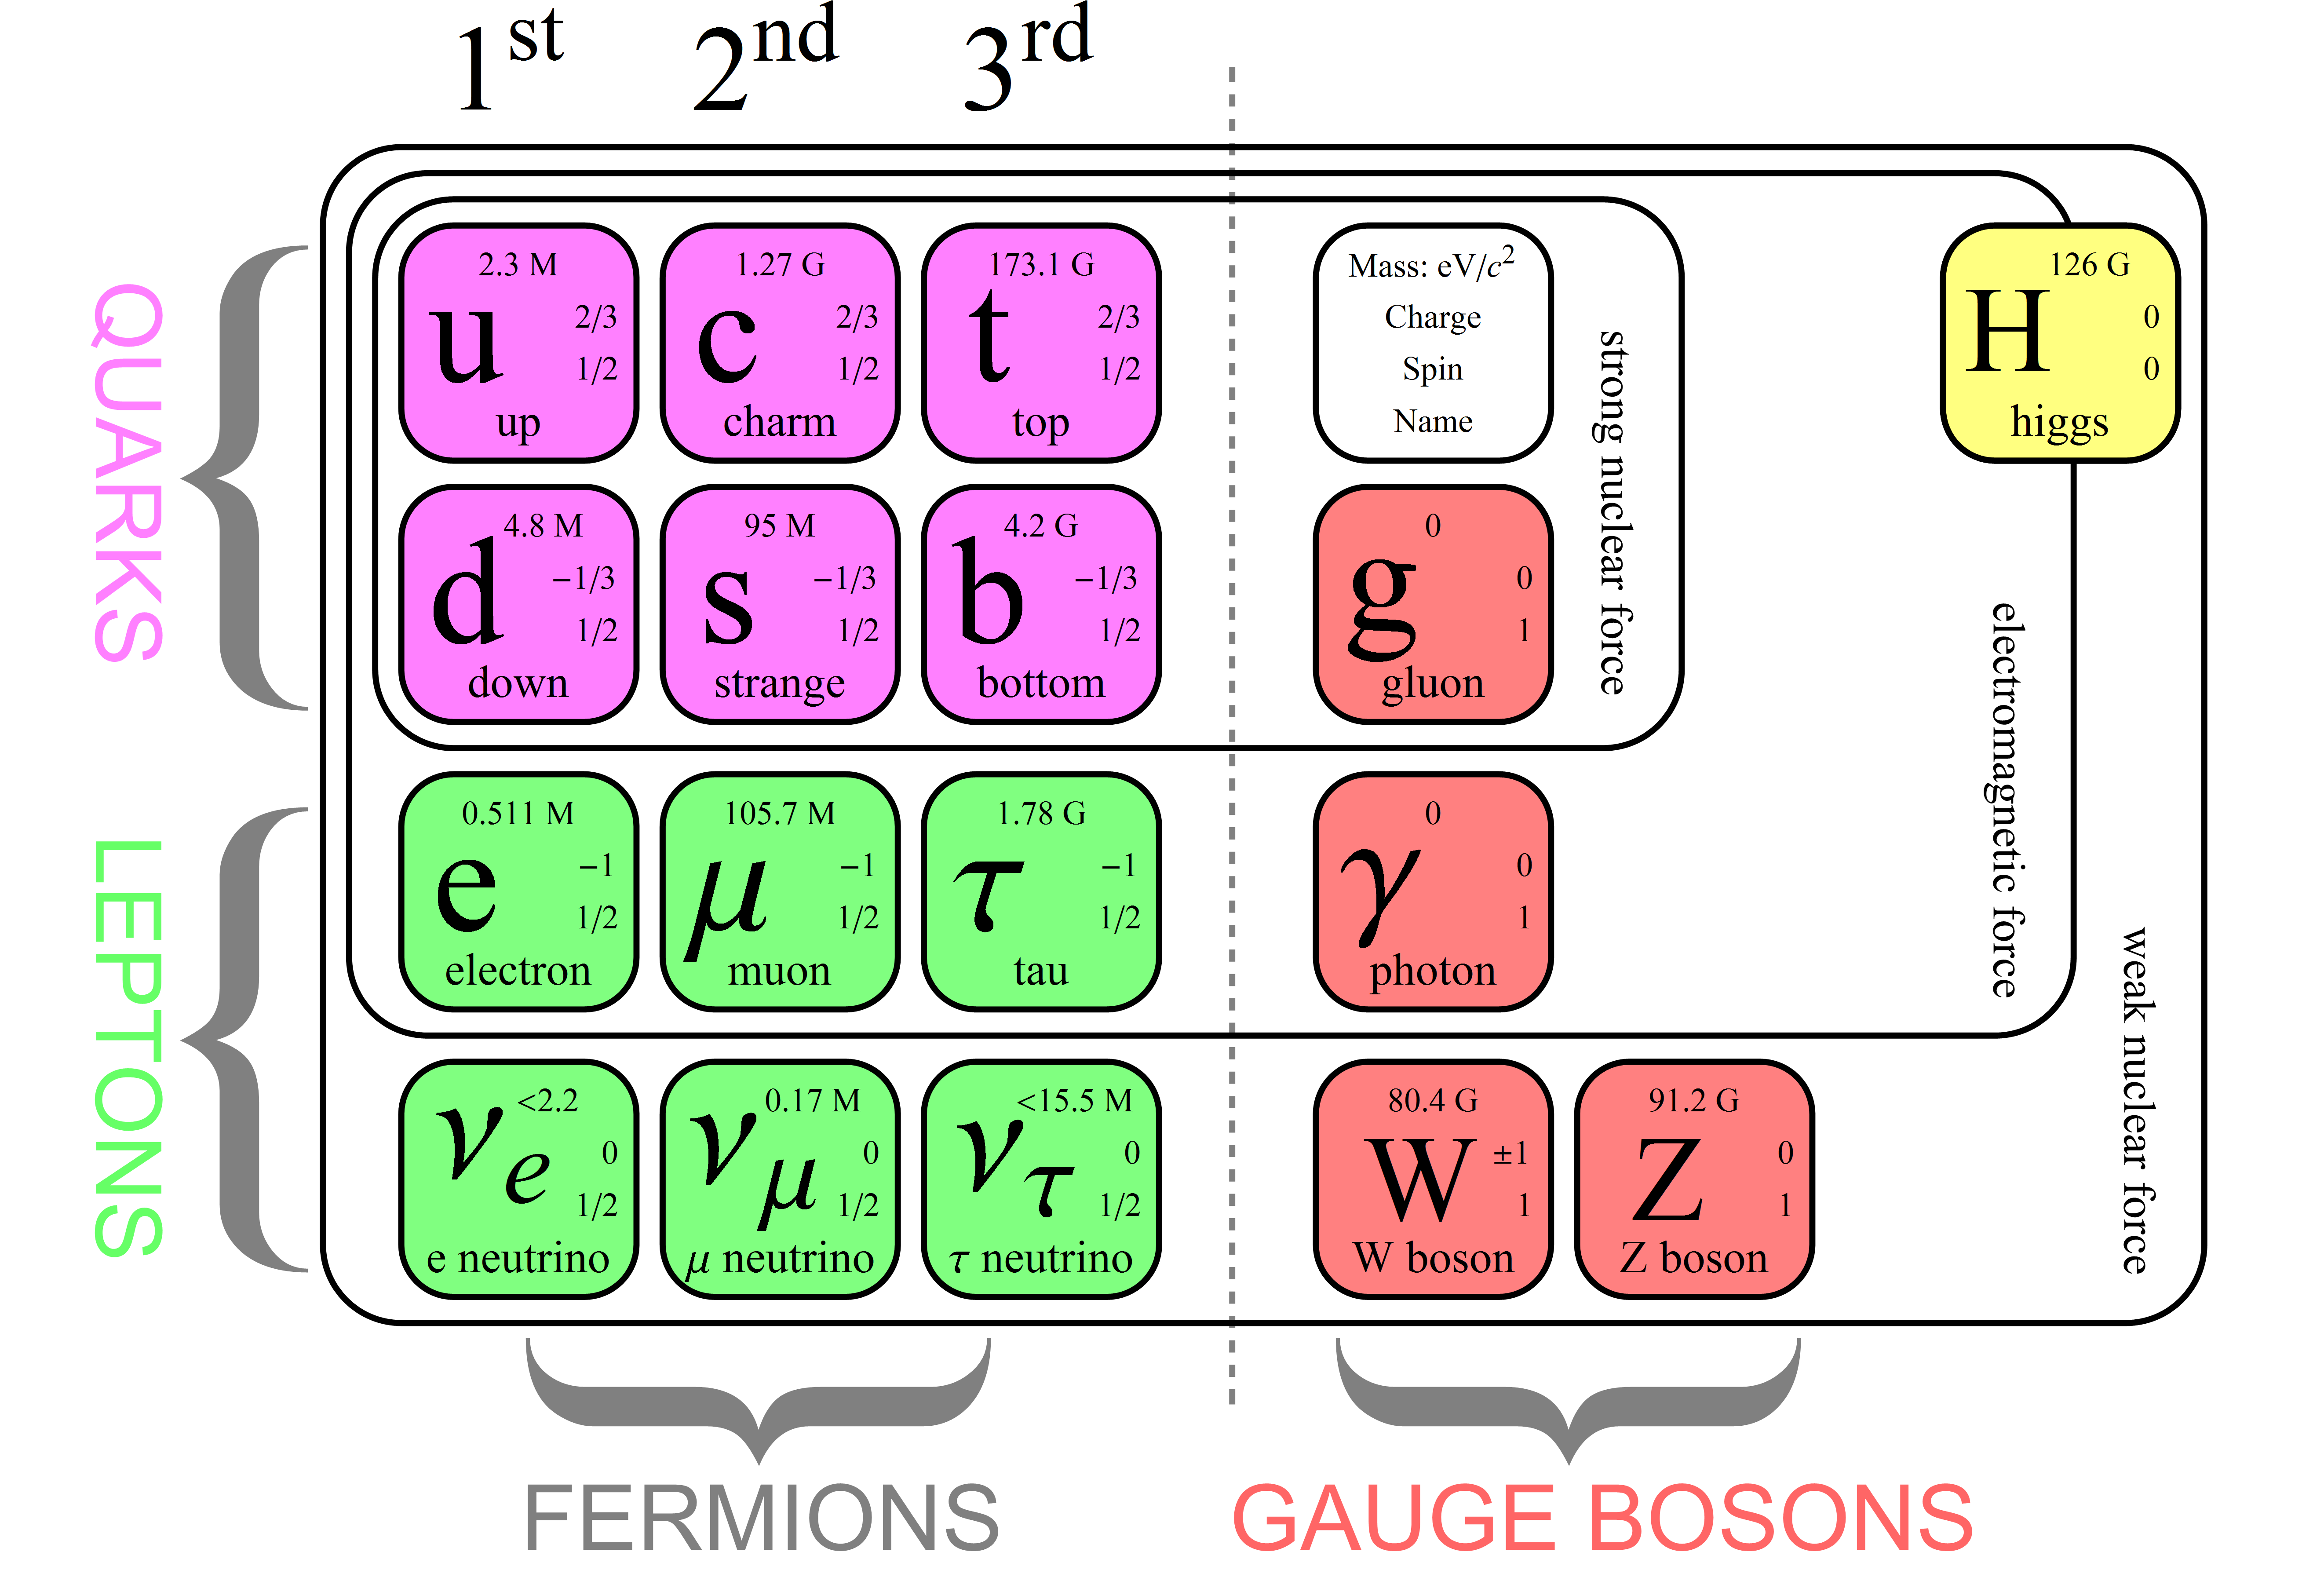
\includegraphics[width=0.98\textwidth]{./plots/SM.png}
  \caption{The particles of the Standard Model.}
  \label{fig:SMParticles}
\end{figure}

\ \\There are 12 fermions representing the constituents of matter. They have a semi-integer spin ($1/2$) and they can be divided into two categories: quarks and leptons. The quarks have fractional electric charges and form barions and mesons. They six quarks are up ($u\,^{+2/3}$), down ($d\,^{-1/3}$), charm ($c\,^{+2/3}$), strange ($s\,^{-1/3}$), top ($t\,^{+2/3}$), and bottom ($b\,^{-1/3}$). The three electrically-charged leptons have a negative charge: the electron ($e\,^{-}$), the muon ($\mu\,^{-}$), and the tau lepton ($\tau\,^{-}$). These have corresponding neutrally-charged leptons caled neutrinos ($\nu_e\,^0$, $\nu_\mu\,^0$, $\nu_\tau\,^0$). These particles form matter. For each matter particle there is an anti-matter particle that has an opposite electric charge. 

\ \\Fermions interact with each other via the echange of other elementary particles called bosons. Bosons are carriers of the elementary forces and have an integer spin ($1$). There are eight type of gluons ($g$) that carry the strong force. The photon ($\gamma$) is responsible for the electromagnetic force. The \Wplus, \Wminus~and the \Zzero~bosons carry the weak force. 

\ \\There is also another type of boson, a scalar elementary particle of spin zero (0), called the Higgs boson. The Higgs boson is the latest elementary particle discovered, in 2012, by the ATLAS and CMS detectors at CERN. It is predicted by the mechanism that explains how the elementary particles acquire mass.

\subsection{The top quark}
\label{sec:TopQuark}

The top quark ($t$) is a very interesting elementary particle to study, for several reasons. It is the heaviest particle from the SM, with a mass \mt=173.3~\GeVcc. This implies the top quark has the highest Yukawa coupling constant. The top quark decays very quickly ($\tau=10^{-25}$ s), before having the time to hadronize, meaning to form stable hadrons. Therefore it is the only quark that can be studied alone. It is observed indirectly through its decay products. The top quark was discovered in 1994 independently by the CDF and DZero experiments at FermiLab in proton-antiproton ($p\bar{p}$) collisions at $\sqrt{s}=1.8$ TeV.

\ \\Measuring the top-quark properties is key to test the validity of the SM. The ATLAS and CMS experiments at CERN measure the properties of the top quark in great detail. If deviations are found in the top quark properties with respect to the SM predictions (\emph{e.g.} different cross-sections), it implies the existence of new physics phenomena beyond the Standard Model (BSM). This would produce a revolution in particle physics, as the SM has not been contradicted by any experiment since its creation in the 1960s. 

\ \\The top quarks are produced in pairs by strong interactions. The Feynman diagrams for the leading order are illustrated in Figure~\ref{fig:TopQuarkFeynmanDiagrams}. At the LHC the quark-antiquark annihilation (left) represents 10\% of the cases, while the gluon-gluon fusion (center and right) represent 90\% of cases. The LHC has a very high luminosity and produces large quantities of top quarks. For this reason the LHC is considered to be also a top-quark factory.

\begin{figure}[h]
  \centering
  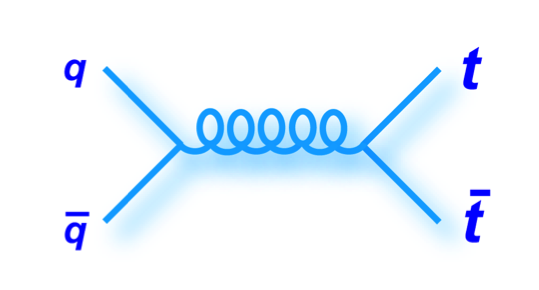
\includegraphics[width=0.32\textwidth]{../presentation/plots/ttbar_1.png}
  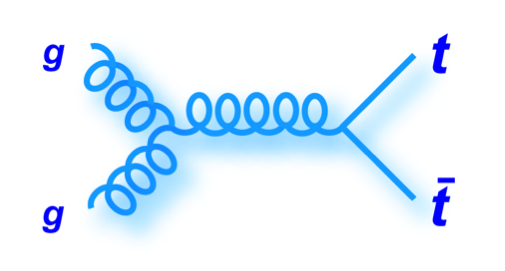
\includegraphics[width=0.32\textwidth]{../presentation/plots/ttbar_2.png}
  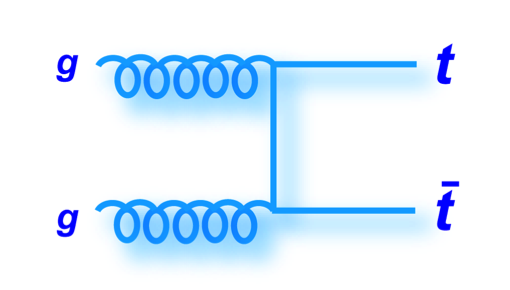
\includegraphics[width=0.32\textwidth]{../presentation/plots/ttbar_3.png}
  \caption{The Feynaman diagrams for the top-quark pair production. At the LHC the quark-antiquark annihilation (left) represents 10\% of the cases, while the gluon-gluon fusion (center and right) represent 90\% of cases.}
  \label{fig:TopQuarkFeynmanDiagrams}
\end{figure}

\ \\The top quark decays in almost 100\% of the time in a \Wboson~and a bottom ($b$) quark. The $W$ boson can decay either to a pair of a quark or an antiquark ($W\rightarrow q\bar{q}$), or to a pair of leptons ($W \rightarrow e\bar{\nu}_e$, $W \rightarrow \mu\bar{\nu}_\mu$, $W \rightarrow \tau\bar{\nu}_\tau$). The $\tau$ lepton decays further leaving as a visible signature in the detector an electron, a muon or two quarks. Since there are two top quarks, they decay to two \Wboson~bosons and two $b$ quarks. Quarks hadronise and appear in the detector as streams of collimated particles called jets. 

\ \\Counting the number of charged leptons (electrons or muons), the top quark events can be grouped into three categories: di-lepton, lepton+jets (one lepton plus jets), and all-hadronic (only jets). The percentage of decay for each case, called branching ratio (BR) is presented in the left-hand side of Figure~\ref{fig:TopQuarkDecay}. In this report we study the subset of the di-lepton with an electron or a muon. The \ttbaremu~decay is present in only 2\% of the cases. It is advantageous because the background is very low comparing to others decay channels. The background comes in most of the cases from the \Zboson~boson decay plus other jets. The full Feynman diagram of production and decay of the \ttbaremu~is presented in the right-hand side of Figure~\ref{fig:TopQuarkDecay}. The latest ATLAS paper on the \ttbaremu~analysis is presented in~\cite{ttbaremu}.

\begin{figure}[h]
  \centering
  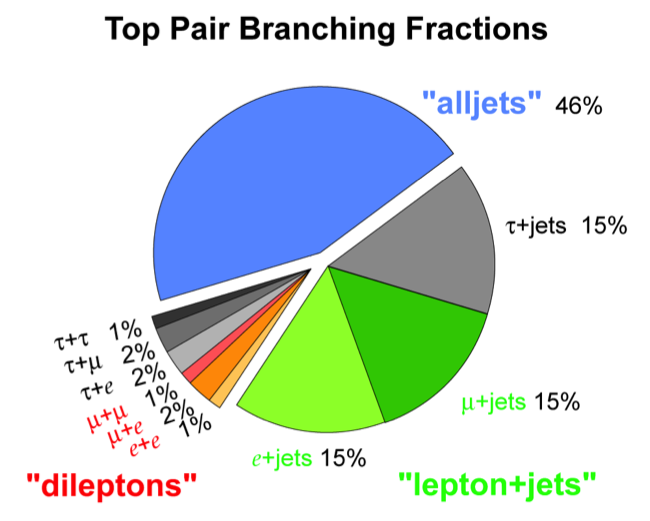
\includegraphics[width=0.47\textwidth]{../presentation/plots/ttbar_5.png}
  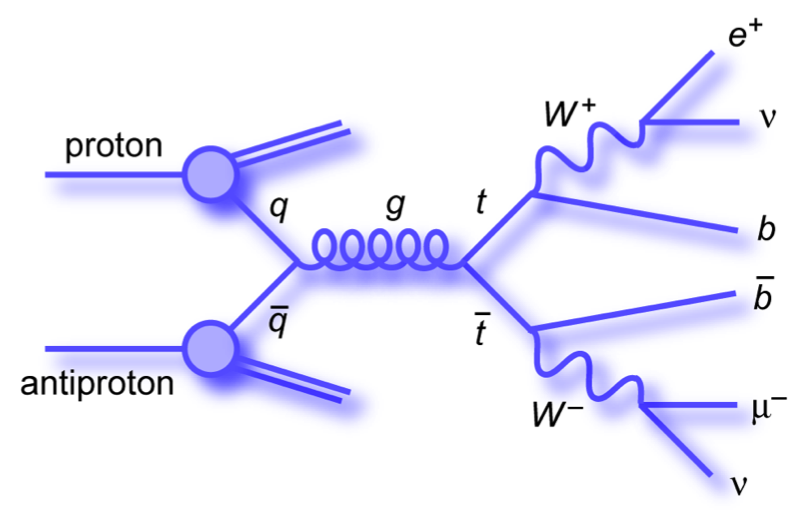
\includegraphics[width=0.47\textwidth]{../presentation/plots/ttbar_4.png}
  \caption{Left: the pie chart of the top-quark pair decay. Right: the Feynman diagram including production and decay of the \ttbaremu~process.}
  \label{fig:TopQuarkDecay}
\end{figure}

\subsection{The experimental setup}
\label{sec:ExperimentalSetup}

The experimental setup used in this study is from the ATLAS experiment at CERN.

\ \\At the moment, the Large Hadron Collider (LHC), which is situated at CERN, is the most powerful proton-proton collider in the world, as illustrated in Figure~\ref{fig:LHC}. After the Tevatron and the Large Electron-Positron Collider (LEP) era, a new machine was needed for new discoveries in particle physics. The LHC was designed to achieve a center-of-mass energy $\sqrt{s}=14\,TeV$. Two of the biggest goals of the LHC are to study the Standard Model and to test its validity.  

\begin{figure}[h]
  \centering
  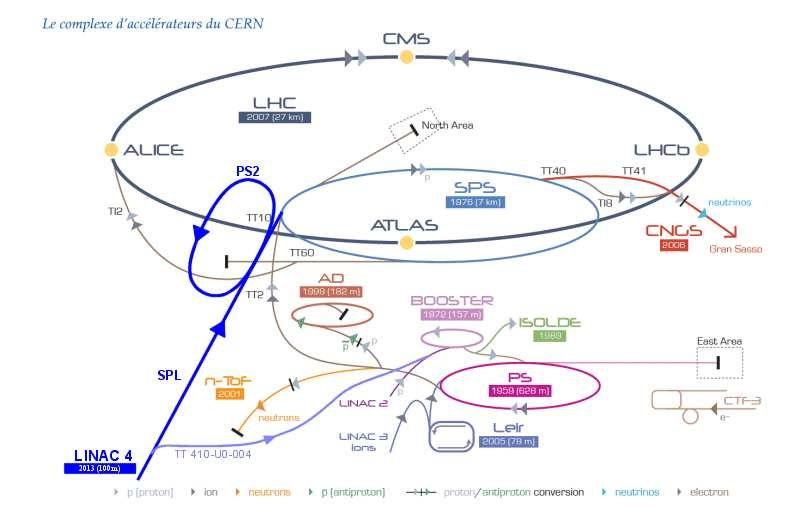
\includegraphics[width=0.5\textwidth]{plots/LHC.png} 
  \caption{The LHC Accelerator Complex System.}
  \label{fig:LHC}
\end{figure}

\ \\This project is affiliated to the international collaboration of the A Toroidal LHC ApparatuS (ATLAS)~\cite{ATLAS}. ATLAS is the largest of the four LHC detectors. ATLAS is one of the two general-purpose particle physics detectors at the LHC, the other being CMS. The two detectors and collaborations perform a similar research program. A new discovery must be observed by both detectors to be believed as true. ATLAS and its subdetectors is illustrated in Figure~\ref{fig:ATLAS}.

\begin{figure}[h]
  \centering
  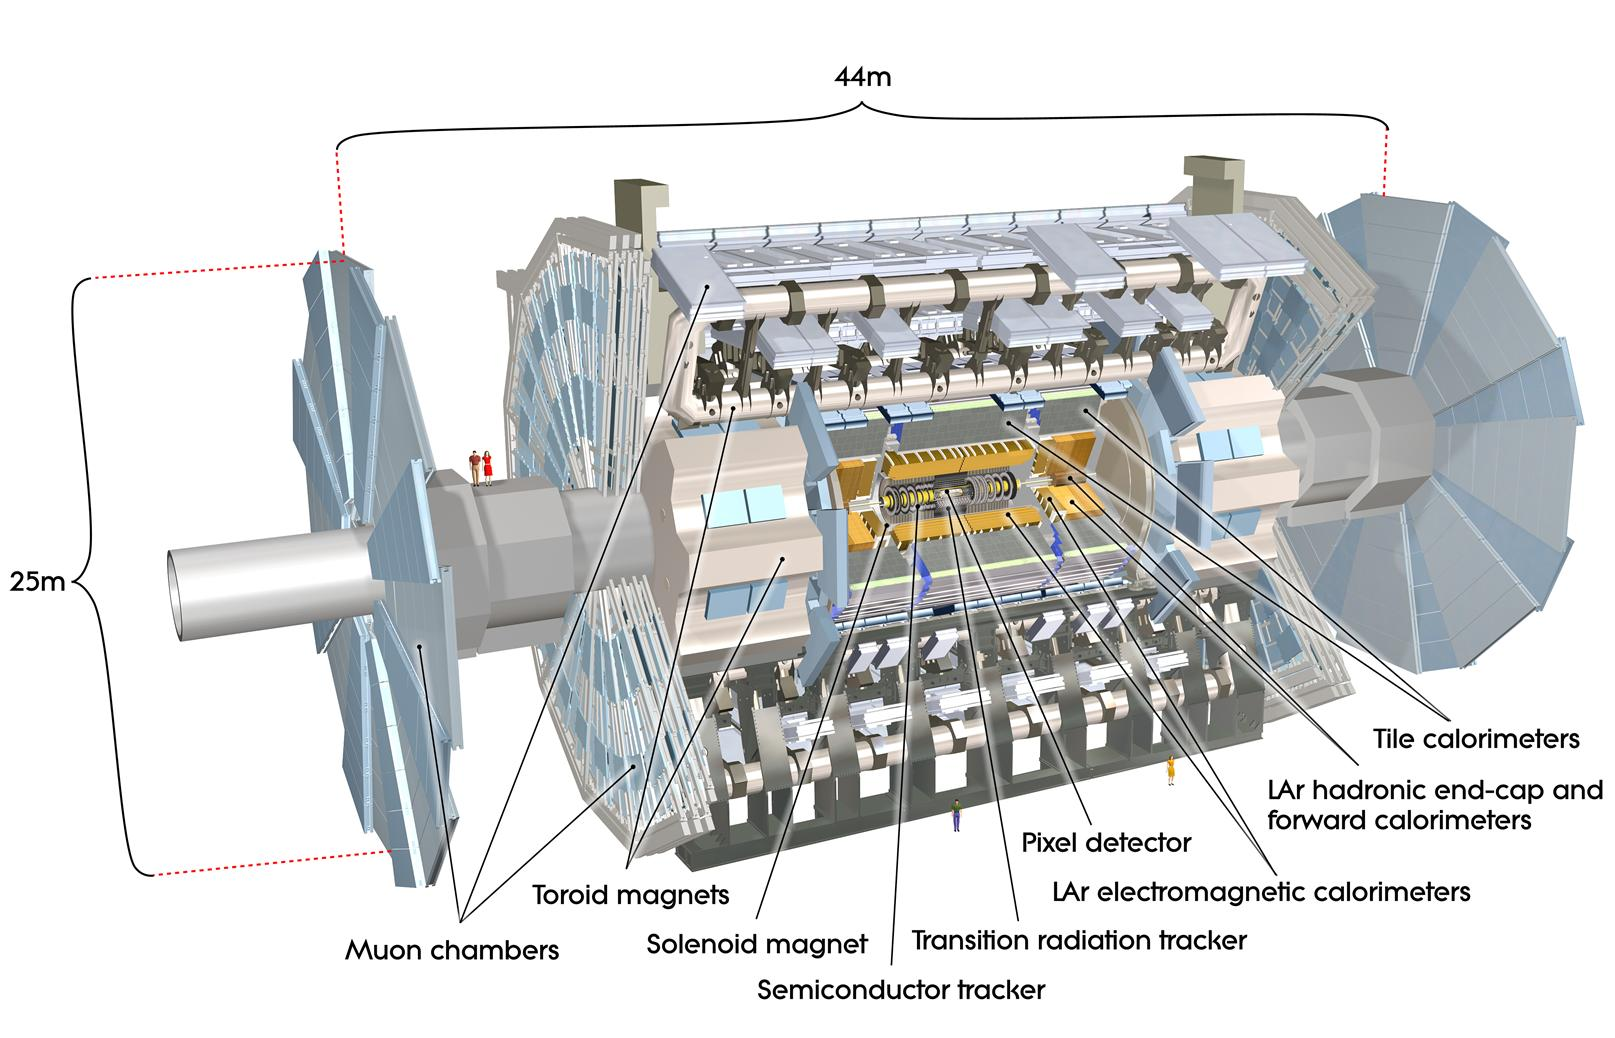
\includegraphics[width=0.5\textwidth]{plots/ATLAS.jpg} 
  \caption{The ATLAS detector and its sub-detectors.}
  \label{fig:ATLAS}
\end{figure}

\ \\ This report presents results obtained using 43076 simulated events of the \ttbaremu~process within the ATLAS experiment~\cite{RootFile}. After an event selection, for each event there is the information available at the reconstructed stage (measured) stage and at the truth (generated) stage. The study focuses on the jet with the highest transverse momentum (\pt), also called the leading jet, in the interval from 0 to 500 \GeV, with a constant bin width of 20 \GeV, which results in 25 bins in total.
